\begin{ParaColumn}[\bisection*{Recent Experimental Data Included in the Database}{数据库中包含的最新试验数据}]
    
    Recently, new large triaxial devices have been operating at École Centrale Nantes (ECN) in France and at the IDIEM laboratory in Chile. The large device at ECN can test samples that are 1,000 mm in diameter and 1,500 mm in height, at a maximum confining pressure of 1.5 MPa. The IDIEM large triaxial device can handle samples of 1,000 mm in diameter and 1,800 mm in height at confining pressures up to 3 MPa. Exhaustive descriptions and testing methodologies can be found in \citet{Hu2011} and \citet{Ovalle2013} for ECN, and in \citet{DelaHozAlvarez2007} for IDIEM.

    \switchcolumn

    最近,新的大型三轴设备已经在法国的南特中央大学(ECN)和智利的IDIEM实验室中投入使用。 ECN的大型设备可以在最大1.5MPa的围压下对直径1000毫米,高度1500毫米的样品进行试验。IDIEM的大型三轴设备可以在最大3MPa的围压下处理直径1000毫米,高度1800毫米的样品。对ECN和IDIEM的详细描述和试验方法可以在\citet{Hu2011}和\citet{Ovalle2013}以及\citet{DelaHozAlvarez2007}中找到。

    \CrossColumnText{
        \begin{figure}[htb]
    \centering
    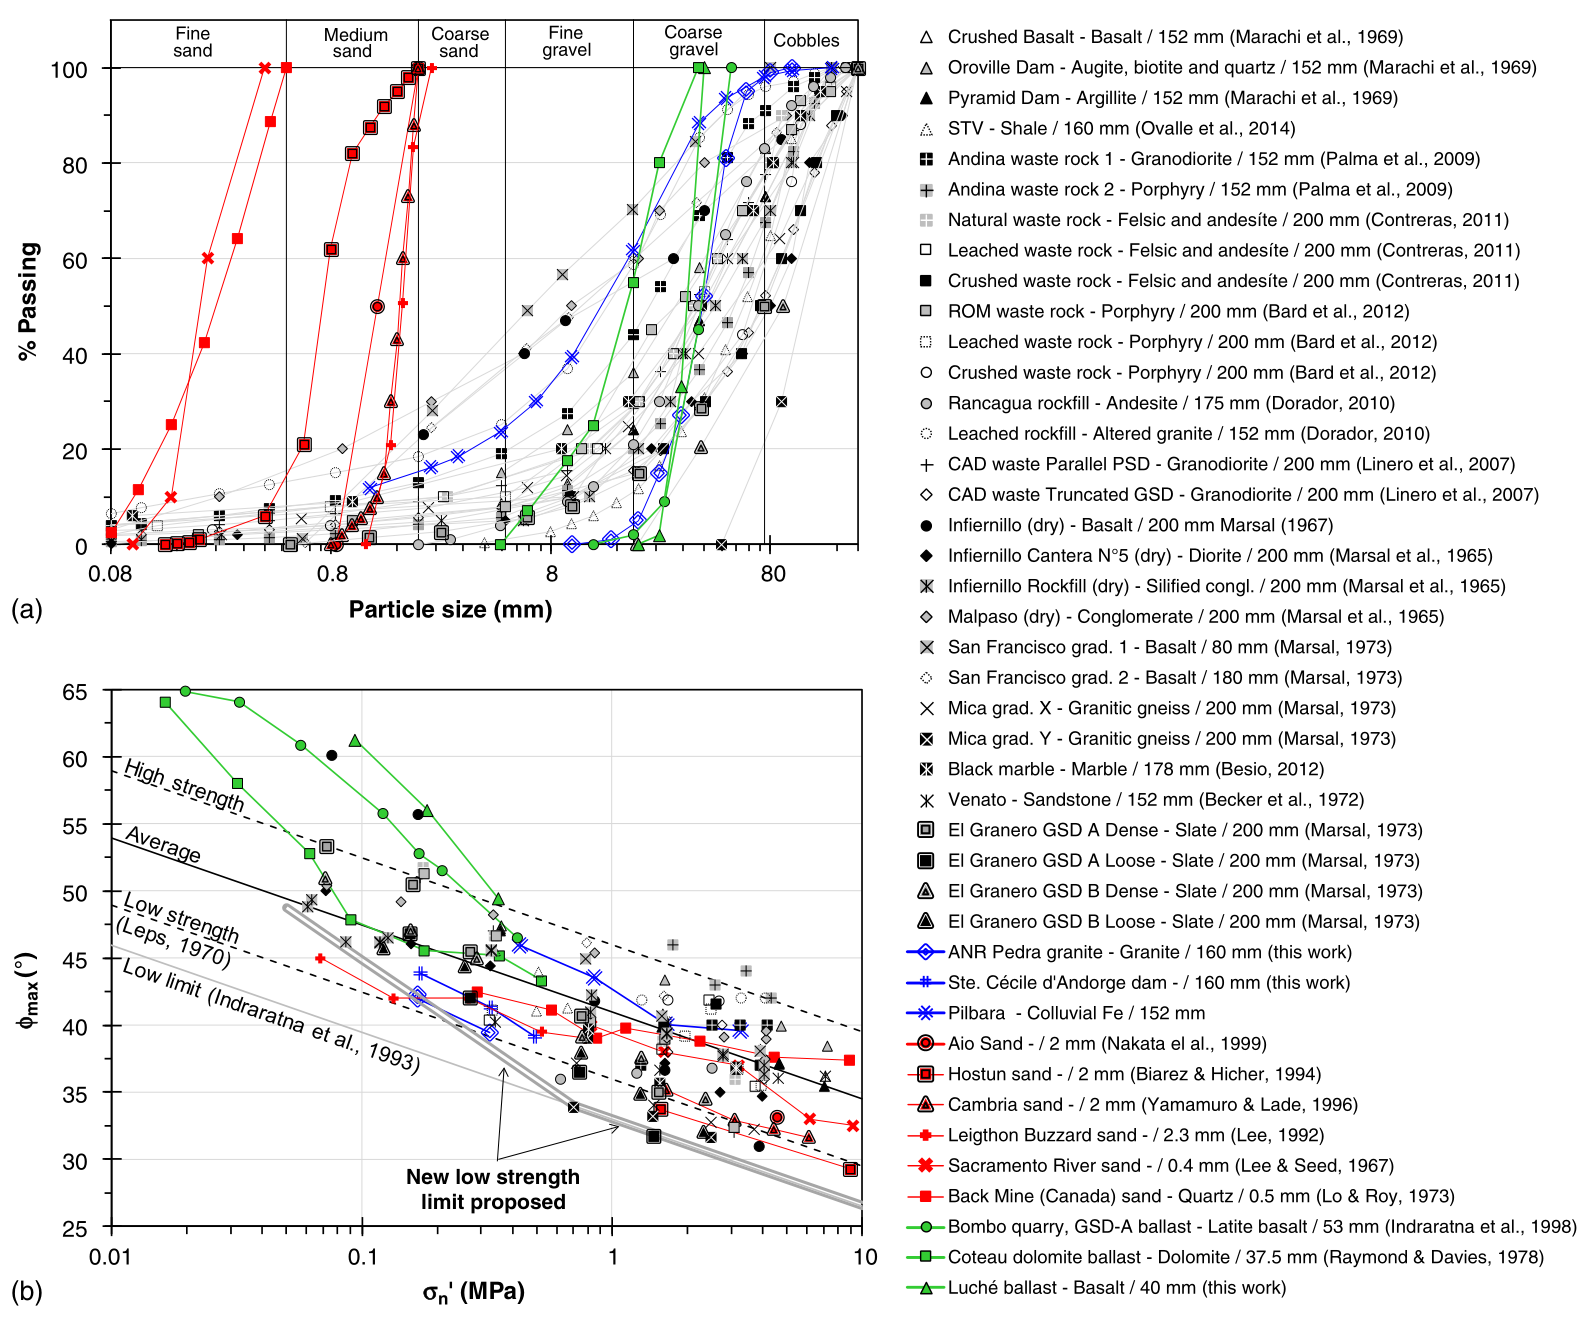
\includegraphics[width=\textwidth]{figures/figure-2.png}
    \bicaption{Compiled sands, ballasts, and rockfills: (a) GSD; and (b) maximum internal friction angle [legend: “Material Name/dmax (millimeters) (Ref.)”]}{汇编的砂土,铁道石渣和碎石料:(a)GSD; (b)最大内摩擦角[图例:“材料名称/$d_{\max}$(毫米)(参考)”]。}
    \label{figure:2}
\end{figure}
    }

    \switchcolumn*

    Among the 158 large triaxial tests on 33 materials compiled and analyzed, 14 rockfill materials were tested at IDIEM (1 unpublished — on Pilbara rockfill), 3 at ECN (2 unpublished — on Agence Nationale de la Recherche (ANR) Pedra granite and Sainte Cécile d’Andorge dam), 4 at UCB, and 12 at CFE. \enautoref{figure:2}(a) shows the grain size distribution (GSD) for each material. Descriptions of the new rockfills reported in this study are the following:

    \switchcolumn

    在已编制分析的33种材料的158个大型三轴试验中,有14种碎石料在IDIEM(1种未发表的Pilbara碎石)上进行了试验,3种在ECN(2种未发表的国家研究机构(ANR)花岗岩和圣塞西尔安道尔大坝),4种在UCB以及12种在CFE上分别进行了试验。 \cnautoref{figure:2}(a)显示了每种材料的颗粒尺寸分布(GSD)。 本研究报告的新碎石场描述如下:

    \switchcolumn*

    \begin{itemize}
        \item \textbf{Pilbara:} Waste crushed mining rockfill from the Pilbara region in Western Australia, consisting of Neogene alluvial and colluvial sediments originated from weathering, erosion, and transportation of Precambrian banded iron formation rocks.
        \item \textbf{ANR Pedra granite:} Washed, crushed angular granite rockfill.\\[-5mm]
        \item \textbf{Sainte Cécile d’Andorge dam:} Schist and mica-schist rockfill with subangular grains.
    \end{itemize}

    \switchcolumn

    \begin{itemize}
        \item \textbf{Pilbara:}来自西澳大利亚Pilbara地区的碎石矿山废碎石,由前寒武纪带状铁地层风化、侵蚀和搬运形成的新近纪冲积、冲积物组成。
        \item \textbf{ANR Pedra花岗岩:}洗碎的有棱角的花岗岩碎石。
        \item \textbf{Sainte Cécile d'Andorge大坝:}带有亚角粒的片岩和云母片岩。
    \end{itemize}

    \switchcolumn*

    The materials analyzed here have diverse origins, and differ in terms of relative density, mineralogy, particle shape, GSD, and water content (tests on saturated and air-dried samples). Accordingly, significant data scatter should be expected. However, due to the lack of available data to perform accurate analyses, this paper aims to present ranges of results for shear strength and secant Young’s modulus to compare the results with quartzitic sands and ballasts and to provide references for engineers and researchers. The analyses presented highlight the influence of the breakage ratio ($B_g$), using the definition of \citet{Marsal196727}, given by the sum of positive differences between the percentage of the total sample contained in each size fraction before and after the test.

    \switchcolumn

    此处分析的材料具有不同的来源,并且在相对密度,矿物成分,颗粒形状,GSD和含水量(在饱和和干燥的样品上进行试验)方面也不同。 因此,预期应该会有大量的数据分散。 但是,由于缺乏准确分析的数据,本文旨在介绍抗剪强度和割线杨氏模量的结果范围,以便与石英砂和铁道石渣进行比较,并为工程师和研究人员提供参考。 本文给出的分析使用\citet{Marsal196727}的定义强调了破损率($B_g$)的影响,该定义由试验前后各尺寸分数中所含总样品百分比的正差之和给出。

\end{ParaColumn}